e\documentclass[12pt,a4paper]{article}
\usepackage[utf8]{inputenc}
\usepackage[bahasa]{babel}
\usepackage{geometry}
\geometry{top=2.5cm, bottom=2.5cm, left=3cm, right=2.5cm}
\usepackage{graphicx}
\usepackage{listings}
\usepackage{xcolor}

% --- Menggunakan Font Times New Roman ---
\usepackage{mathptmx} 

\definecolor{codegreen}{rgb}{0,0.6,0}
\definecolor{codegray}{rgb}{0.5,0.5,0.5}
\definecolor{codepurple}{rgb}{0.58,0,0.82}
\definecolor{backcolour}{rgb}{0.95,0.95,0.92}

\lstset{
  backgroundcolor=\color{backcolour},   
  commentstyle=\color{codegreen},
  keywordstyle=\color{blue},
  numberstyle=\tiny\color{codegray},
  stringstyle=\color{codepurple},
  basicstyle=\ttfamily\small,
  breakatwhitespace=false,         
  breaklines=true,                 
  captionpos=b,                    
  keepspaces=true,                 
  numbers=left,                    
  numbersep=5pt,                  
  showspaces=false,                
  showstringspaces=false,
  showtabs=false,                  
  tabsize=4,
  language=C++
}


\title{\textbf{Laporan Praktikum C++}}
\author{Wisam Yassar Mahardika}
\date{\today}

\begin{document}

\maketitle

\section{Penamaan Variabel yang Benar dan Salah}

\subsection{Penamaan Variabel Salah (Error)}
\begin{lstlisting}
  // Bagian ini akan error jika dicompile langsung
  int float;
  float int;
  string 2kata;
  double int;
  bool @asdf;
\end{lstlisting}

\subsection{Penamaan Variabel Benar}
\begin{lstlisting}
  #include <iostream>
  using namespace std;

  int main() {
    int jumlah;
    float outputSensor;
    string namaOrang;
    bool status;
    double temperatur;
    return 0;
  }
\end{lstlisting}

\section{Deklarasikan Tipe}
\begin{lstlisting}
  #include <iostream>
  using namespace std;

  int main() {
    int jumlahPerangkat = 10;
    double suhuTerbaca = 23.12;
    bool statusRelayMenyala = false;
    string namaLengkapPerangkat = "DHT11";
    return 0;
  }
\end{lstlisting}

\section{Program Identitas}

\subsection{Kode Sumber Utama}
\begin{lstlisting}
  #include <iostream>
  using namespace std;

  int main() {
    string nama, alamat;
    int usia, tinggi, berat;
    
    cout << "Masukan Nama: ";
    cin >> nama;
    cout << "Masukan Usia: ";
    cin >> usia;
    cout << "Masukan Alamat: ";
    cin >> alamat;
    cout << "Masukan Tinggi: ";
    cin >> tinggi;
    cout << "Masukan Berat Badan: ";
    cin >> berat;
    
    cout << "Nama anda adalah: " << nama << endl
    << "Usia anda adalah: " << usia << endl
    << "Alamat anda adalah: " << alamat << endl
    << "Tinggi anda adalah: " << tinggi << endl
    << "Berat badan anda adalah: " << berat << endl;
    return 0;
  }
\end{lstlisting}

\subsection{Hasil Output}
\begin{figure}[h]
  \centering
  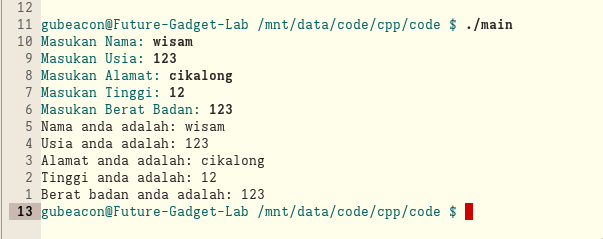
\includegraphics[width=0.8\textwidth]{screenshotwell.png}
  \caption{Tampilan Output Program Identitas}
  \label{fig:output}
\end{figure}

\end{document}
